\documentclass[talk.tex]{subfiles}
\begin{document}


    	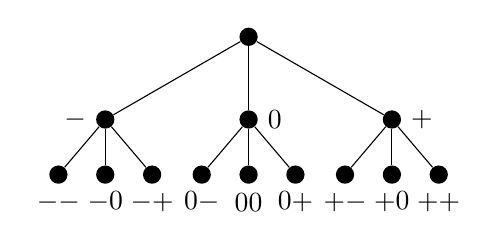
\begin{tikzpicture}[scale=.35,
    	 grow=down,
    	 level 1/.style={sibling distance=5.2cm, level distance=3cm}, 
    	 level 2/.style={sibling distance=1.7cm, level distance=2cm},
    	 level 3/.style={level distance=1cm}]
    	 
    	 % style of the vertices
    	 \tikzstyle{vertex}=[circle,fill,scale=0.7]
    	 
			\node [vertex] {}
				child {node [vertex, label=left:$-$] {}
					child {node [vertex] {}
						child {node {$--$} edge from parent[draw=none] }}
					child {node [vertex] {}
						child {node {$-0$} edge from parent[draw=none] }}
					child {node [vertex] {}
						child {node {$-+$} edge from parent[draw=none] }}}
				child {node [vertex, label=right:0] {}
					child {node [vertex] {}
						child {node {$0-$} edge from parent[draw=none] }}
					child {node [vertex] {}
						child {node {$00$} edge from parent[draw=none] }}
					child {node [vertex] {}
						child {node {$0+$} edge from parent[draw=none] }}}
				child {node [vertex, label=right:$+$] {}
					child {node [vertex] {}
						child {node {$+-$} edge from parent[draw=none] }}
					child {node [vertex] {}
						child {node {$+0$} edge from parent[draw=none] }}
					child {node [vertex] {}
						child {node {$++$} edge from parent[draw=none] }}};
    		
		\end{tikzpicture}

\end{document}